%% ------------- English version ---------------
\documentclass[english,hidelinks]{sbrt}
\usepackage{newtxtext}
\usepackage[english]{babel}
\usepackage[utf8]{inputenc}
%% ---------------------------------------------
\usepackage{hyperref}
\usepackage{amsmath}
\usepackage{graphicx}
\graphicspath{{figs/}{./}}
\usepackage{tikz}
\usetikzlibrary{arrows.meta,positioning}
\usepackage[
  compatibility=false,
  font=footnotesize,
  labelsep=period,
  format=plain,
  justification=raggedright,
  singlelinecheck=false
]{caption}

\begin{document}

\title{Smartphone-Assisted Calibration of a Two-Screen Display for Head-Coupled Perspective Rendering}

\author{Ewerton Arrais, Miguel Veiga, Emilly Fernandes and Rigel Fernandes}

\maketitle

\markboth{XLV BRAZILIAN SYMPOSIUM ON TELECOMMUNICATIONS AND SIGNAL PROCESSING - SBrT 2027}{}

\begin{abstract}
Head-coupled perspective turns a screen into a window onto a 3D scene by redrawing it from the viewer's eye position. Using two screens requires the pose of the second screen relative to the first with millimeter accuracy. This paper presents a system that obtains this pose from about twelve photographs taken with an ordinary smartphone. Each screen displays a ChArUco board whose metric size follows from the panel dimensions; the photographs calibrate the phone camera and give one pose estimate per photograph, and a bundle adjustment enforces a single screen pose and also estimates the size of the second screen. A notebook webcam tracks the viewer and both screens are rendered with an off-axis projection. On real photographs, the bundle adjustment reduced the variation of the estimated screen corners across photograph subsets from 2.5~mm to 0.4~mm.
\end{abstract}
\begin{keywords}
Multi-screen calibration, fish tank VR, ChArUco markers, bundle adjustment, head-coupled perspective.
\end{keywords}

\section{Introduction}

Flat displays show a scene from a fixed viewpoint, so the image does not change when the viewer moves. Head-coupled perspective, or fish tank virtual reality, tracks the viewer's head and redraws the scene from that viewpoint, so that the screen behaves like a window; Ware et al.~\cite{ware1993fish} showed that the resulting motion parallax is a strong depth cue on an ordinary monitor. The rendering uses an off-axis projection whose parameters depend on the physical position of the screen and of the eye, as formalized by Kooima~\cite{kooima2009generalized}.

Extending the effect to several screens enlarges the virtual space, but the pose of every screen must then be known in a common frame: an error of a few millimeters appears as a break at the seam between screens. Fafard et al.~\cite{fafard2017calibration} point to this calibration as the obstacle to multi-screen fish tank displays, and Wagemakers et al.~\cite{wagemakers2017interactive} calibrate such displays visually, by having the user align patterns across the seams, assuming the screen geometry is already known.

Low-cost vision systems based on facial landmarks and commodity cameras have been used for driver fatigue detection~\cite{assumpcao2025fatigue} and for liveness monitoring in remote work~\cite{gama2025liveness}. The same kind of landmark model~\cite{grishchenko2020attention} can supply the eye position that head-coupled rendering needs, with no dedicated tracking hardware.

This work proposes a system that recovers the pose of an external monitor relative to a notebook screen from photographs taken with a smartphone, and uses it to render one shared 3D world on both screens. The contributions are: (i) the screens themselves act as calibration targets, and the phone camera is calibrated from the same photographs; (ii) a bundle adjustment that enforces one screen pose for all photographs and estimates the unknown size of the monitor; (iii) a two-screen head-coupled renderer with a correction for head yaw; and (iv) an evaluation that compares the bundle adjustment with per-photograph averaging on simulated and real photographs. The source code is available in~\cite{parallax2026repo}.

The rest of this work is organized as follows. Section~\ref{sec:II} describes the system. Section~\ref{sec:III} details the proposed method. Section~\ref{sec:IV} reports the results, and Section~\ref{sec:V} concludes the work.

\section{System Description}
\label{sec:II}

The system uses two cameras and no microcontroller. The notebook webcam ($1280\times720$~px) is the tracking sensor: it is fixed to the notebook screen, which defines the world frame. The smartphone camera is used only during calibration. The phone opens a web page served by the notebook, reached through a QR code shown on the screen; each photograph is taken with the native camera application and uploaded over HTTP, on the local network or through an SSH tunnel when the devices cannot reach each other. The page reports how many board corners were found in each photograph, so a bad photograph is rejected immediately.

The software is written in Python. OpenCV~\cite{bradski2000opencv} provides image capture, 2D drawing, the ArUco detector~\cite{garrido2014automatic} and camera calibration; MediaPipe provides the face landmark model~\cite{grishchenko2020attention}; NumPy and SciPy provide linear algebra and the least-squares solver. The projection, the scenes, the bundle adjustment, the photograph simulator and the user interface were implemented by the authors. The problem addressed is the one stated above: finding, with equipment a user already owns, the rigid transform between the two screens that the off-axis projection requires.

\section{Proposed Method}
\label{sec:III}

Fig.~\ref{fig:pipeline} summarizes the method. The upper part runs once and produces the calibration file; the lower part runs at every frame.

\begin{figure}[t]
\centering
\tikzset{
  box/.style={draw, rounded corners=1.5pt, align=center, font=\scriptsize, inner sep=2.5pt, text width=7.0cm},
  arr/.style={-{Stealth[length=1.6mm]}, semithick}
}
\begin{tikzpicture}[node distance=2.2mm]
\node[box] (a) {ChArUco board on each screen (metric size from the panel)};
\node[box, below=of a] (b) {Smartphone photographs of both screens};
\node[box, below=of b] (c) {Corner detection; phone camera calibration from the same photographs};
\node[box, below=of c] (d) {Pose of each screen per photograph (PnP); robust mean};
\node[box, below=of d] (e) {Bundle adjustment: one monitor pose and monitor size};
\node[box, below=of e, fill=black!8] (f) {Calibration file (pose of the monitor in the notebook frame)};
\node[box, below=of f] (g) {Webcam: iris landmarks, eye position, yaw correction, filter};
\node[box, below=of g] (h) {Off-axis projection on each screen, shared draw order};
\foreach \x/\y in {a/b,b/c,c/d,d/e,e/f,f/g,g/h} \draw[arr] (\x) -- (\y);
\end{tikzpicture}
\caption{Proposed method: calibration (top) and per-frame rendering (bottom).}
\label{fig:pipeline}
\end{figure}

\subsection{Targets and Metric Scale}
Each screen displays a $13\times7$ ChArUco board drawn at one board pixel per screen pixel, with marker identifiers 0--44 on the notebook and 45--89 on the monitor, so every detected corner is attributed to its screen. The physical side of a square is its size in pixels times the pixel pitch, given by the screen width divided by its horizontal resolution. The notebook screen is the only ruler of the system; for the monitor, only its nominal diagonal is supplied, as an initial value.

\subsection{Detection and Phone Calibration}
In each photograph the ArUco markers~\cite{garrido2014automatic} are detected, the chessboard corners are interpolated and refined to subpixel accuracy, and corners inconsistent with a homography fitted by RANSAC are discarded. The intrinsic parameters of the phone camera (focal lengths, principal point and two radial distortion coefficients) are estimated from these same detections by the planar method of Zhang~\cite{zhang2000flexible}, with each pair (photograph, screen) as one view. No separate calibration session is needed.

\subsection{Per-Photograph Pose and Robust Mean}
The pose of each board in each photograph is obtained by solving the Perspective-n-Point problem with the planar solver of Collins and Bartoli~\cite{collins2014infinitesimal}, refined by Levenberg--Marquardt. For a photograph $k$ that shows both screens, the pose of the monitor $M$ in the notebook frame $N$ is
\begin{equation}
T^{(k)}_{N\leftarrow M} = \big(T_{C_k\leftarrow N}\big)^{-1}\,T_{C_k\leftarrow M},
\label{eq:pair}
\end{equation}
in which the camera pose $C_k$ cancels, so the phone can be held freely. The estimates are combined by the chordal mean of the rotations and the median of the translations, after discarding outliers. This estimator, called PnP+mean, is the baseline.

\subsection{Bundle Adjustment}
\label{sec:ba}
PnP+mean treats the photographs independently. The proposed estimator imposes that the screens do not move between photographs. A bundle adjustment~\cite{triggs2000bundle} estimates one monitor pose $T_{N\leftarrow M}$, the pose of every photograph, the camera intrinsics and a scale factor $\sigma$ for the monitor size, minimizing the reprojection error of all corners,
\begin{equation}
\min \sum_{k}\sum_{s}\sum_{m} \rho\!\left(\big\|\pi\big(T_{C_k\leftarrow N}\,T_{N\leftarrow s}\,X_{sm}(\sigma_s)\big)-u_{ksm}\big\|^2\right),
\label{eq:ba}
\end{equation}
where $s\in\{N,M\}$, $\pi$ is the camera projection with distortion, $X_{sm}$ the metric position of corner $m$ on screen $s$, $u_{ksm}$ its detection, $T_{N\leftarrow N}=I$ and $\sigma_N=1$. The problem is solved by sparse nonlinear least squares, first with a quadratic loss and then with the Huber loss $\rho$, starting from PnP+mean. The monitor size is observable because viewpoints at different positions remove the ambiguity between a larger, farther screen and a smaller, closer one.

\subsection{Tracking and Two-Screen Rendering}
The face landmark model returns the centers of both irises. With a pinhole model and an interpupillary distance of 64~mm, the iris distance in pixels gives the distance to the camera, $Z=f\,\mathrm{IPD}/d_{px}$, and the midpoint gives $X$ and $Y$; the webcam focal length $f$ is measured once, with the viewer at a known distance. Looking at the side monitor turns the head, which shortens the iris distance in the image and would overestimate $Z$ by about 15\% at $30^\circ$. The head rotation returned by the landmark model gives the 3D direction $a$ of the line between the eyes, and the position is multiplied by $k=\|a_{xy}-a_z\,n\|$, where $n$ is the normalized image position of the midpoint. The position is smoothed with a One Euro filter~\cite{casiez2012oneeuro}.

Each scene point is drawn where the line from the eye to the point crosses the screen plane, which is equivalent to the off-axis projection of~\cite{kooima2009generalized}. For the monitor, the eye and the scene are first expressed in its frame using the calibrated pose. Polygons are clipped by the plane of each screen and painted back to front in an order computed once in the world frame, so occlusion agrees on both sides of the seam.

\section{Results and Discussion}
\label{sec:IV}

\subsection{Setup and Qualitative Results}
The prototype, shown in Fig.~\ref{fig:setup}, uses a notebook with a 15.6-inch screen ($1920\times1080$~px, $345.4\times194.3$~mm) and a 23-inch external monitor at its left. Twelve photographs of $4080\times3072$~px were taken with a Google Pixel 7 Pro from different positions; all twelve showed both boards, with 72 corners detected per screen in most of them. The calibration placed the monitor at $27.8^\circ$ from the notebook screen, with a 3.3~cm gap between the inner edges. Fig.~\ref{fig:planet} shows a scene rendered on both screens with this calibration: a ringed planet behind the seam, half on each screen. The sphere and the rings are continuous across the seam only if the estimated pose is correct. An alignment scene with straight rods crossing the seam provides the same visual check. Rendering both screens takes 11 to 17~ms per frame, below the period of the webcam, which limits the loop to about 20~frames per second.

\begin{figure}[t]
\centering
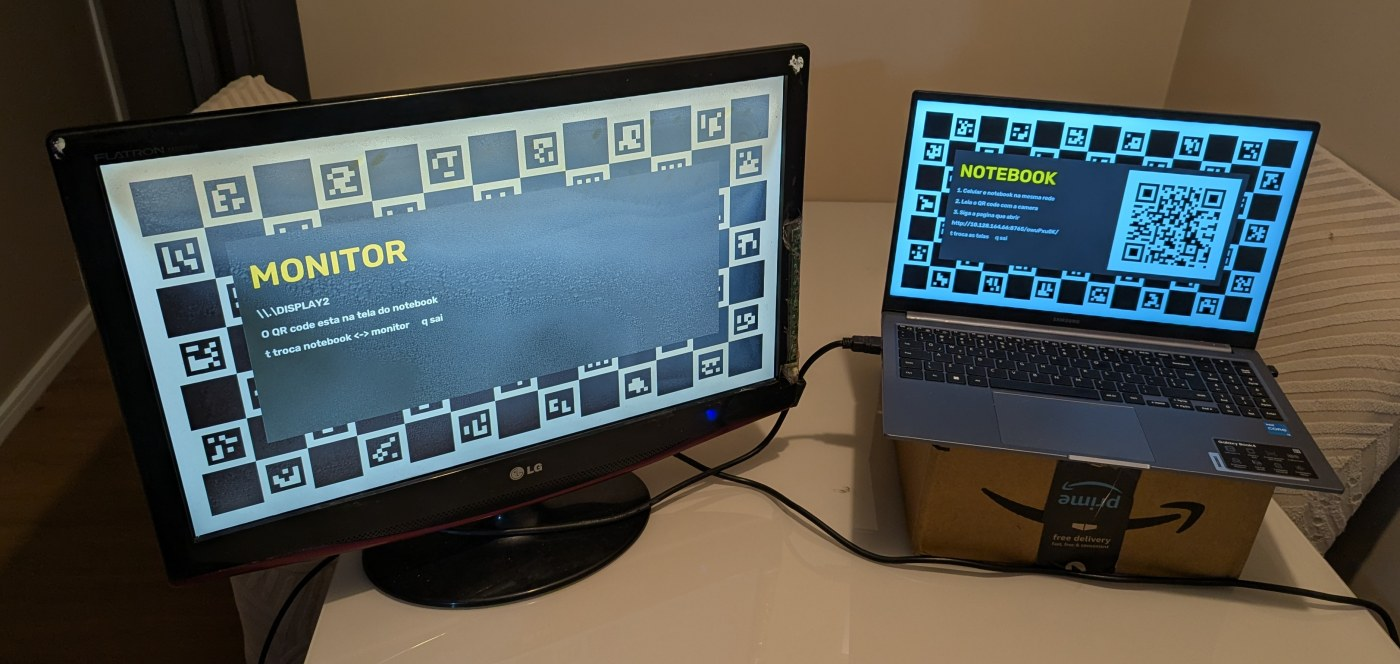
\includegraphics[width=0.92\columnwidth]{fig_setup.jpg}
\caption{Prototype during calibration: ChArUco boards on the monitor and on the notebook, and the QR code that opens the capture page on the phone.}
\label{fig:setup}
\end{figure}

\begin{figure}[t]
\centering
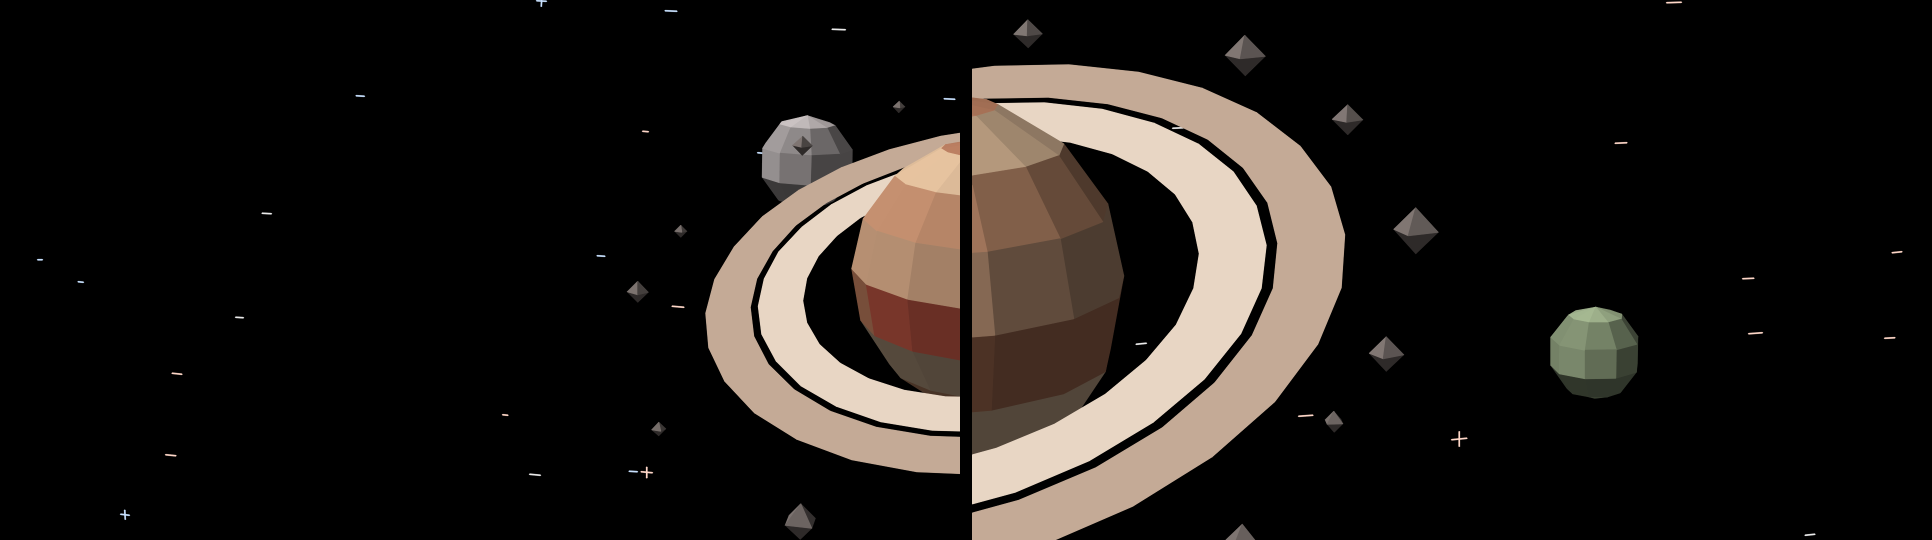
\includegraphics[width=\columnwidth]{fig_planet.png}
\caption{Scene rendered on the monitor (left) and on the notebook (right) with the calibration from real photographs.}
\label{fig:planet}
\end{figure}

\subsection{Quantitative Results}
Three estimators are compared: PnP+mean, the bundle adjustment with the monitor size given (BA) and with the size estimated (BA+size). On simulated photographs with known ground truth, generated with blur, sensor noise, moir\'e, glare and JPEG compression at two severity levels, the metric is the largest position error among the four monitor corners, over five sets of ten photographs. On the real photographs there is no ground truth, so the metric is repeatability: each estimator is run on 30 random subsets of ten photographs and the deviation of the monitor corners from their mean is reported.

\begin{table}[t]
\centering
\footnotesize
\caption{Comparison of the estimators. Simulated: worst-corner error, median (maximum). Real: deviation of the corners across subsets, standard deviation (maximum). Values in mm.}
\label{tab:results}
\setlength{\tabcolsep}{4pt}
\begin{tabular}{lccc}
\hline
Photographs & PnP+mean & BA & BA+size \\
\hline
Simulated, typical & 0.21 (0.53) & 0.11 (0.16) & 0.23 (0.32) \\
Simulated, poor    & 0.47 (1.01) & 0.16 (0.21) & 0.22 (0.26) \\
Real, 12 photos    & 2.5 (5.5)   & 0.7 (2.3)   & 0.4 (1.2) \\
\hline
\end{tabular}
\end{table}

Table~\ref{tab:results} lists the results. In simulation the bundle adjustment reduces the maximum error from 1.01 to 0.21~mm with poor photographs, and estimating the monitor size costs about 0.1~mm. On the real photographs the difference is larger: the corners vary by 2.5~mm with PnP+mean and by 0.4~mm with BA+size. Here BA+size is the best estimator because the nominal diagonal supplied for the monitor (24~inches) was wrong: the adjustment estimated $51.0\times28.7$~cm, which matches the $509\times286$~mm that the monitor itself reports to the operating system. The root-mean-square reprojection error was 1.13~px (0.86~px on the notebook and 1.35~px on the monitor, whose panel is damaged). The yaw correction was verified numerically on 2000 synthetic head poses, where it recovers the distance exactly, but its gain was not measured on a real face, and the calibration was not compared with a tape measure; these are limitations of the present evaluation.

\section{Conclusion}
\label{sec:V}

This work presented a system that calibrates the geometry of a two-screen display with photographs from an ordinary smartphone and uses it for head-coupled perspective rendering. The screens act as calibration targets, the phone camera is calibrated from the same photographs, and a bundle adjustment yields a single pose and the size of the second screen. On real photographs it reduced the variation of the estimated monitor corners from 2.5~mm, with per-photograph averaging, to 0.4~mm, and recovered the true size of a monitor whose nominal diagonal had been entered incorrectly. The complete system, from the capture page on the phone to the two-screen renderer, runs on a notebook with its built-in webcam. As future work, we intend to compare the calibration with physical measurements, to measure the yaw correction on real faces, and to extend the calibration to more than two screens and to screens outside the direct view of the phone.

\bibliographystyle{ieeetr}
\bibliography{refs}

\end{document}
